% Number 960
% CAPMG CVPMG Units 
% Drag racer - CAPM and CVPM - graphical
% JG

% Watermark
\AddToShipoutPicture*{\BackgroundPic}

\addtocounter {ProbNum} {1}

%\begin{floatingfigure}[r]{.44\textwidth}
%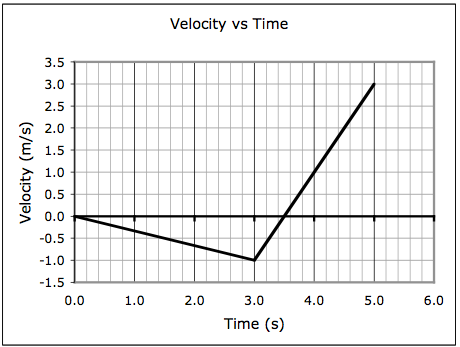
\includegraphics[scale=.54]{/Users/jgates/desktop/latex/pics/vgraph6}
%\end{floatingfigure}
 
{\bf \Large{\arabic{ProbNum}}} A drag racer begins at rest, and accelerates to ${140~\tfrac{m}{s}}$ within 2.1 seconds.  Once at this speed, the racer maintains it through the finish line, which is 400 meters from the start line. \bigskip

Draw position, velocity, and acceleration graphs for this motion, with accurate values on all axes.  Make sure to denote the time at which the racer finishes the race.
\vfill


%\begin{center}
%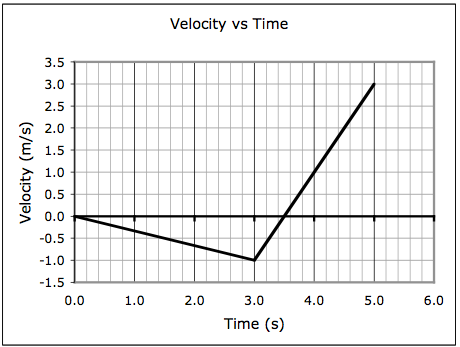
\includegraphics[scale=1]{/Users/jgates/desktop/latex/pics/vgraph6}
%\end{center}


\newpage